In this study, an agent-based model simulates the pollination of plants in a forest using two interacting agents; one mobile agent, \emph{pollinators or animals} and one static, \emph{plants}.  To determine how genes flow we keep track of the order of the plants each pollinator interacts with to determine the likely genetics of the seed creation.  Next we discuss the specific rules used in the model.
%We consider different plant densities to examine what effect density has on the distribution of
%pollen.  Plants have a limited supply of pollen that can be gathered by pollinators.  Pollinators in turn
%transport pollen across the landscape using a corrolated random walk.  At each step, pollinators examine the local neighborhood for plants
%where they will collect and deposit pollen.

\subsection{Movement}

Movement in the model is done by the pollinators, which carry pollen from one plant to another.
Each step of the pollinator's movement is conducted in two stages: \emph{searching} and \emph{movement}.
First, the pollinator checks a neighborhood of radius $r$ to see if there are any plants within the neighborhood.
If there are one or more plants, the pollinator chooses the closest.  It there are two or more that are
equidistant from the pollinator, one is randomly chosen.

If there are no plants within a distance $r$ from the current location of the pollinator, the pollinator
moves according to a correlated random walk.  For the correlated random walk, the direction is chosen
based on a probability distribution centered about
its current direction, see \autoref{Figangle}.  In the simulations we vary the maximum turning angle (AMT) {\bf Erich-Why didn't we call it MTA instead)}.  We relate the strength of the correlated random walk with the size of the turning angle.  So for a purely random walk AMT is $180^{\circ}$ and there would be no correlation, and as AMT decreases the correlation grows stronger.  {\bf Erich-purely random diffusion should be true for the uniform distribution but not the normal distribution, what are the results in the graphs using?}

The pollinator then takes a step with
length between 0 and 1 distributed uniformly in the new chosen direction.  This length is denoted by
$s_j^{(i)}$, which is the $j^{th}-$step taken by the $i^{th}$ pollinator.\\
\vspace{.8in}

\begin{figure}[h!]\label{TurningAngle}
\begin{center}
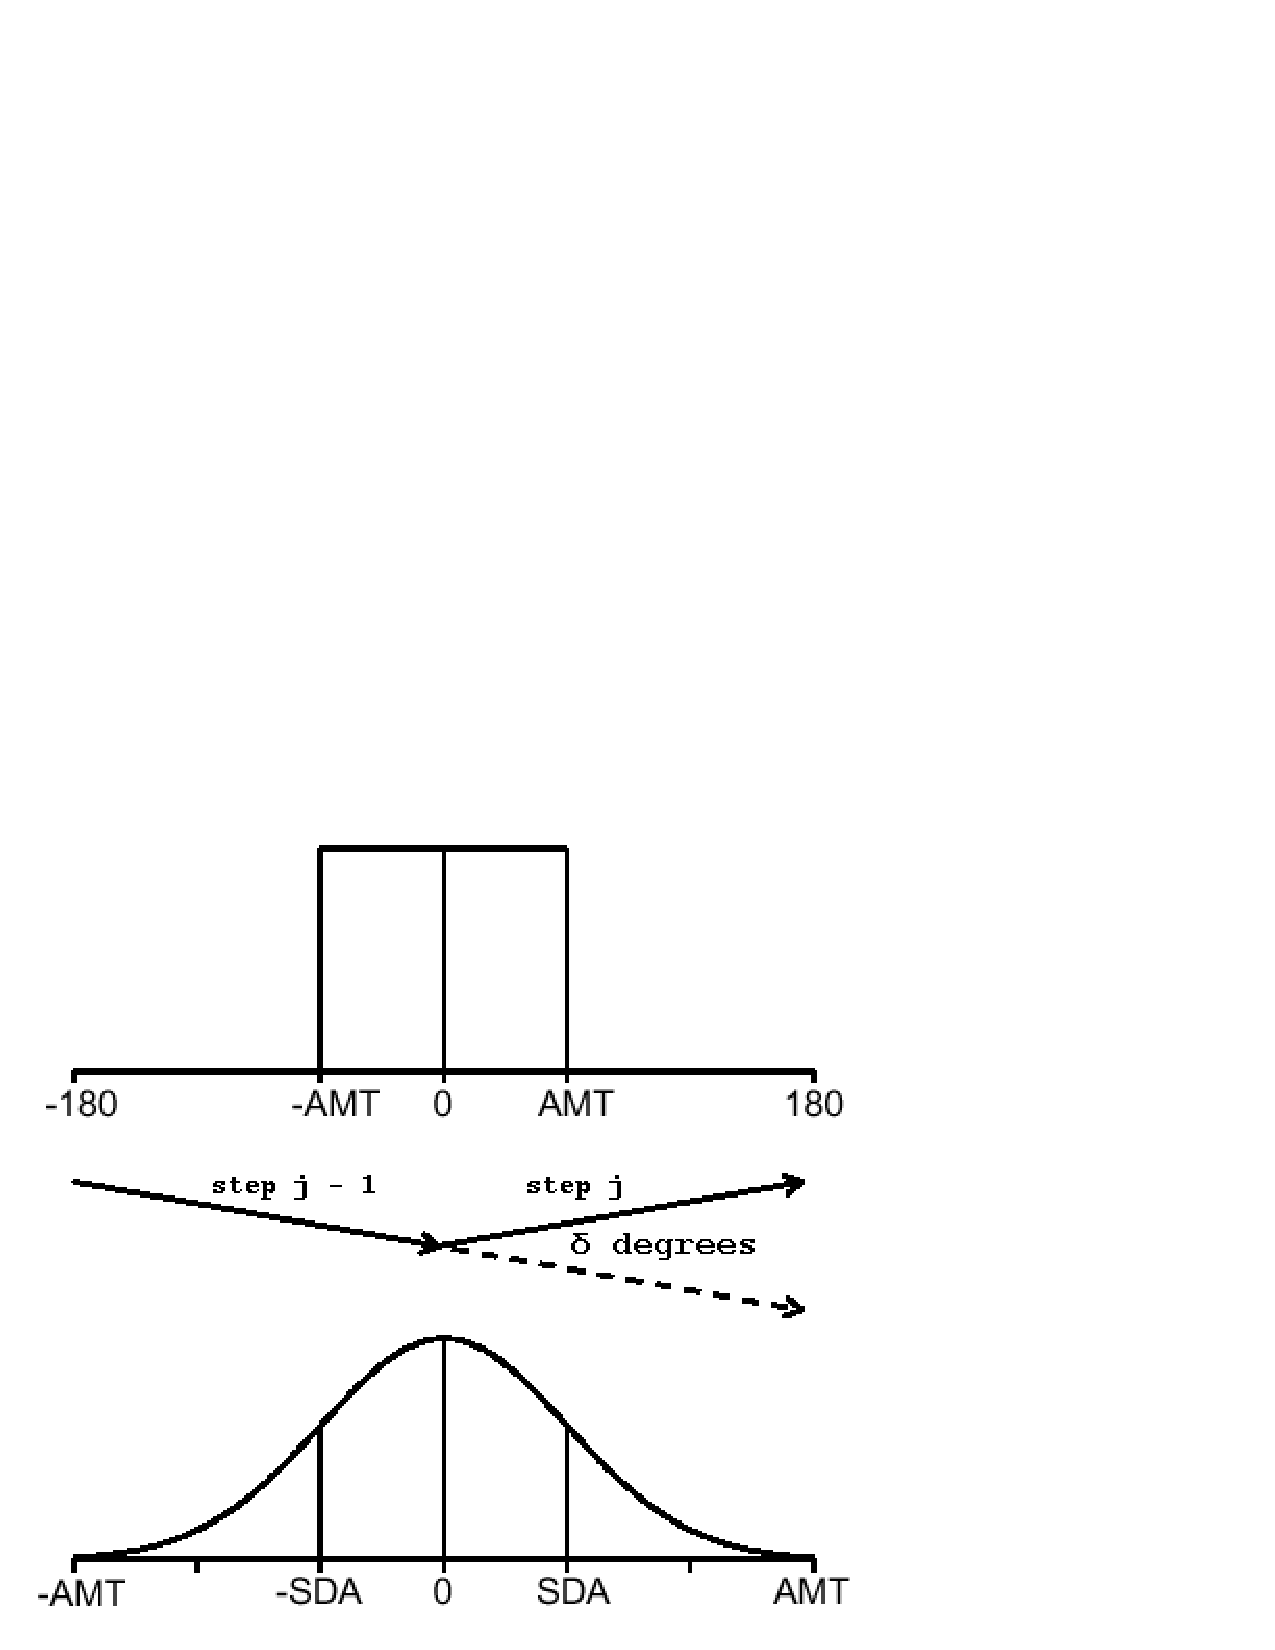
\includegraphics[scale=0.5,trim=0 30 150 510]{TADistribution.pdf}
\end{center}
\caption{Turning Angle for (a) uniform distribution and (b) depiction
of what a path may look like.}
\label{Figangle}
\end{figure}
{\bf Erich-Maybe in this figure we should just use the uniform distribution?}


Alternatively, if the pollinator is already at a plant, the pollinator picks a random direction uniformly
and takes a step with length $r+1$ distributed uniformly.  This will ensure that the pollinator will not immediately return to
the same plant on the next step.

\subsection{Pollination}

When an pollinator is on a plant, it collects pollen, distributes pollen, and consumes food. Each
plant has a particular number of flowers, $\phi$, from which an pollinator may obtain pollen. When an pollinator
visits a plant it picks up pollen from one or more flowers. The number of flowers from which an
pollinator can obtain pollen is determined by the total number of flowers on a plant, the fraction of
flowers in bloom at any one time ($a$), the number of times ($j$) the plant has previously been
visited by an pollinator, and the maximum fraction of flowers available for pollination ($\eta$). The
formula for the number of total flowers available for visitation during a $k^{th}$ visit to the
$j^{th}$ plant ($f_{j,k}$) is given by

\begin{equation}\label{flowers}
f_{j,k} = \phi \cdot a \cdot \eta^k.
\end{equation}

The amount of food eaten and the amount of pollen collected is proportional to
the number of visited flowers. Pollinators collect and eat pollen from each flower they
visit.  The amount of pollen collected and the amount of food eaten is proportional to the
equation \eqref{flowers}. Let $f^{\left(i\right)}_{j,k}$ be the number of flowers visited by the
$i^{th}$ pollinator during the $k^{th}$ visit to the $j^{th}$ plant, then the amount of pollen consumed
by the $i^{th}$ pollinator after $m$ plant visits is given by
\begin{equation}
c^{\left(i\right)}_m = \sum_{j=0}^{m} \beta f^{\left(i\right)}_{j,k},
\label{limit}
\end{equation}
where $\beta$ is the proportionality constant for the amount of pollen collected at a plant.
Each pollinator has a maximum amount of food they will ingest, $c_{max}$, where if they eat that much food they will stop
searching. %The total amount of food that an pollinator can eat is limited
%by the stomach size, $c_{max}$.

The fraction, $\alpha$, of all flowers are pollinated, and the associated probability that a
flower is pollinated, $\rho$, are related by the equation,
\begin{equation} \label{Prob}
\alpha = \rho \cdot \hat{f}_k.
\end{equation}
Using equation \eqref{limit} and \eqref{Prob} we can determine the probability that a flower is
pollinated, $\rho$, by the formula
\begin{equation*}
\rho = \frac{\alpha}{\phi} \cdot \frac{1 - \eta}{a \cdot \eta}.
\end{equation*}
To determine where the pollen originated when a flower is pollinated, we consider each flower previously visited but exclude those flowers from the same plant as the flower being pollinated.    Self-pollination, is not considered, since the likelihood of
self-pollination is low due to mechanisms that impedes self-pollination. Each other flower considered
has an equal likelihood of pollinating the current flower, and a flower is chosen at random.

\subsection{Time and Stopping Criteria}

The speed a pollinator travels ($v$) is constant, as well as the time spent on a
plant ($t_{plant}$).  The travel time for an pollinator is then given by the formula
\[
t^{\left(i\right)} = \frac{s^{\left(i\right)}}{v} + T^{\left(i\right)} \cdot t_{plant},
\]
where $T^{\left(i\right)}$ is the number of plants visited by the $i^{th}$ pollinator. If we let the
maximum allowable travel time be $t_{max}$, then once $t^{\left(i\right)} \geq t_{max}$ or
$c^{\left(i\right)}_m \geq c_{max}$ the pollinator is removed from the simulation. $t_{max}$ is based
on the optimal searching time during the day.  When the pollinator leaves the simulation, it is terminated.

\subsection{Model Statistics}

To best explore the inherent differences between biotic and abiotic pollination this study focuses
on the effects of the strength of the correlated random walk as well as the effects of plant density.

\begin{table}[h]
\setlength{\extrarowheight}{10pt}
{\footnotesize
\begin{tabular}{|l|l|}
  \hline
  % after \\: \hline or \cline{col1-col2} \cline{col3-col4} ...
  Measure & Equation \\[8pt] \hline   \hline
  Average Path Distance & $\bar{s} = \frac{1}{b} \sum_{i=1}^b \sum_{j=1}^n s^{\left(i\right)}_j$ \\[8pt] \hline
  Average Maximum & $ \bar{M} = \frac{1}{b} \sum_{i=1}^b \max_j \sqrt{\left(x^{\left(i\right)}_{1,0}
- x^{\left(i\right)}_{1,j}\right)^2 +
      \left(x^{\left(i\right)}_{2,0} -
x^{\left(i\right)}_{2,j}\right)^2}  $ \\[8pt]
 Distance & \\ \hline
  Average Pollination  & $ \bar{p} = \frac{1}{n} \sum_{i=1}^{n} \left(
\frac{1}{\tau^{\left(i\right)}} \sum_{j=1}^{\tau^{\left(i\right)}}
\sqrt{\left(x^{\left(i\right)}_1 -
x^{\left(j\right)}_1\right)^2 + \left(x^{\left(i\right)}_2 -
    x^{\left(j\right)}_2\right)^2}
    \right)  $ \\[12pt]
    Distance & \\ \hline
  Average Maximum  & $ \bar{P} = \frac{1}{n} \sum_{i=1}^{n} \max_j \sqrt{\left(x^{\left(i\right)}_1 -
x^{\left(j\right)}_1\right)^2 + \left(x^{\left(i\right)}_2 -
    x^{\left(j\right)}_2\right)^2}$ \\[8pt]
   Pollination Distance & \\ \hline
  Average Weighted   & $ E = \frac{1}{n} \sum_{i=1}^n 1/\frac{1}{\left(\tau^{\left(i\right)}\right)^2}
  \sum_{j=1}^{\Delta\tau^{\left(i\right)}} F^2_{j,i} $ \\[8pt]
  Diversity of Fathers & \\
  \hline
\end{tabular}
}
\caption{Equations}
\label{tab:eqn}
\end{table}

We calculate \emph{Average Path Distance} and \emph{Average Maximum Distance}, which are based upon the pollinators' movement and gives a sense how this movement differs with changes in density and the maximum turning angle.  We also calculate
\emph{Average Pollination Distance}, \emph{Average Maximum Pollination Distance}, and \emph{Average
Weighted Diversity of Fathers}, which are based on the pollination events occurring in the model.  These give a more direct results in how gene flow is affected in the model.
The calculations of these statistics are given in the \autoref{tab:eqn}.

In these equations it is assumed that $b$ is the number of pollinators, $n$ is the total number
of plants, $(x_{1,0}^{(i)},x_{2,0}^{(i)})$ is the starting location of the $i^{th}$ pollinator,
$(x_{1,j}^{(i)},x_{2,j}^{(i)})$ is the location of the $i^{th}$ pollinator after $j$ steps,
$\tau^{(i)}$ is the total number of seeds for the $i^{th}$ plant, $\Delta\tau^{(i)}$ is the number
of different fathers contributing pollen to the $i^{th}$ plant, and $F_{j,i}$ is the number of
times the $j^{th}$ father contributed pollen to the $i^{th}$ plant.

